\section{Implementazione}
\label{sec:chapter_navigazione_scena_implementazione}

Il navigatore è stato creato utilizzando il linguaggio Javascript ed in particolare la libreria Three.js.
\\
La scena 3D viene disegnata grazie ad un oggetto Renderer a cui viene assegnato una canvas della grandezza dello schermo dove viene mostrato l’ambiente da visitare.
\\
Il renderer creato utilizza la scena caricata tramite file .json ed una PerspectiveCamera per effettuare la renderizzazione durante la modalità in prima persona e dall’alto.
\\
La scena viene importata grazie all’utilizzo dell’oggetto THREE.ObjectLoader che permette di effettuare il parsing del formato di scambio JSON4.
Durante il parsing vengono riconosciute tutte le strutture dati Three.js da caricare.
\\
Il parser è stato modificato nel presente lavoro di tesi in modo tale da permettere il riconoscimento delle informazioni riguardanti le CubeMap e le env-map che altrimenti non sarebbe stato possibile riconoscere.
\\
Le informazioni delle env-map vengono calcolate immediatamente dopo che la scena è stata completamente caricata. La scena caricata proviene dal servizio di baking che ha applicato ad essa le lightmap, le env-map invece non vengono generate dal servizio ma direttamente dal navigatore.
\\
Questo permette di risparmiare i dati delle immagini delle env-map cubiche, quindi sei immagini per cubo, durante lo scambio dei dati. Immagini che appesantirebbero enormemente la grandezza del json.
\\
Vengono quindi ricreate le informazioni delle CubeCamera, prelevate le sei immagini che rappresentano l’env-map e quindi assegnate all’oggetto corretto. Viene inoltre riconosciuto il tipo di mapping delle CubeCamera, se di riflessione o rifrazione in modo da generare correttamente l’effetto di riflessione o rifrazione sull’oggetto a cui è assegnata l’env-map.
\\
L’oggetto a cui viene applicato l’effetto, a differenza degli altri presenti nella scena, deve essere necessariamente costituito da un materiale di tipo \texttt{MeshBasic} in quanto nell’ambiente caricato sono totalmente assenti fonti luminose. Questo tipo di materiale infatti non viene influenzato dalle luci nella scena e permette di osservare l’oggetto a cui viene assegnato anche in assenza di esse. Quindi durante il parsing, quando viene riconosciuto un oggetto a cui è associata una env-map, ad esso viene assegnato un materiale di tipo MeshBasic.

Durante la navigazione dell’alto viene sfruttata la libreria THREE.TrackballControls, che permette di modificare la camera a piacimento in base al movimento del mouse, trackpad o touch. Durante la navigazione in prima persona è stata utilizzata la libreria \texttt{THREE.PointerLockControls}.
\\
Quest’ultima è stata utilizzata come punto di partenza e poi completamente ristrutturata e modificata per permettere costruire un algoritmo di navigazione in prima persona estremamente preciso e fluido con caratteristiche uniche.
Inoltre i PointerLockControls comportano alcuni problemi nella fluidità dei movimenti dell’osservatore e problemi nella posizione dell’osservatore quando i controlli vengono messi in pausa.
\\
Quando questo accade, la posizione dell’osservatore viene infatti spostata inspiegabilmente in un punto differente da quello in cui si trovava prima della pausa. Problema risolto, salvando in memoria l’ultima posizione dell’osservatore prima di entrare di bloccare la navigazione in prima persona.
\\
Il PointerLockControls deve essere correttamente configurato per permettere un tipo di navigazione che riproduca in maniera credibile una passeggiata all’interno dell’ambiente.
Inoltre non permette la gestione delle collisioni, funzionalità essenziale in questo elaborato e che ha richiesto un approfondito studio e sperimentazioni al fine di costruire un algortimo efficiente che la permettesse.
\\
Durante l’algoritmo delle collisioni viene utilizzata la libreria \texttt{threeoctree.js} per la suddivisione dello spazio e viene utilizzata la classe Raycaster per permettere di gestire le intersezioni dei raggi lanciati con gli oggetti.
\texttt{Octree} permette di dividere lo spazio in cubi; l’algoritmo inizia a dividere da un nodo radice che costituisce un cubo che circonda l’intero ambiente.
\\
Successivamente questo nodo viene ulteriormente suddiviso in 8 parti. Le divisioni continuano dividendo ogni cubo presente in 8 parti fino a quando una soglia di suddivisione massima non viene raggiunta \cite{octree}.

\begin{figure}[htb]
 \centering
 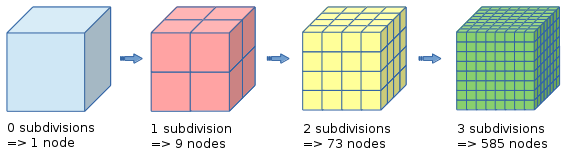
\includegraphics[width=1\linewidth]{images/chapter_navigazione_scena/full_octree.png}\hfill
 \caption[Octree e la suddivisione dello spazio.]{La suddivisione dello spazio tramite Octree.}
 \label{fig:navigazione_scena_collision_full_octree}
\end{figure}

Octree suddivide il volume in 8 parti solamente quando è necessario, come osservabile in figura \ref{fig:navigazione_scena_collision_full_octree}.

L’algoritmo prova sempre a dividere un nodo in 8 nodi, quando però all’interno del nodo non sono presenti triangoli che occupano quello spazio allora esso non viene suddiviso. 
Questo permette di appesantire inutilmente le operazione da effettuare durante il partizionamento.
\\
Nell’esempio sono presenti due sfere su due lati opposti del cubo.  Nella prima divisione, il mondo viene suddiviso in 2 nodi e non in 8. 
\\
Questo perché le sfere risiedono in soli due nodi.
Se viene effettuata la divisione altre due volte, i cubi vengono nuovamente creati solamente vicino alle sfere. L’algoritmo quindi permette la creazione di nuovi nodi solamente dove ce n’è bisogno.

\begin{figure}[htb]
 \centering
 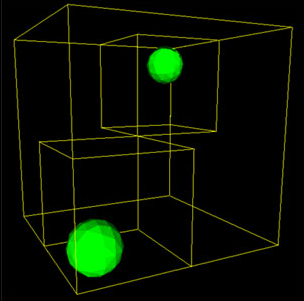
\includegraphics[width=0.6\linewidth]{images/chapter_navigazione_scena/div_2sfere.png}\hfill
 \caption[Octree e la suddivisione dello spazio.]{La suddivisione dello spazio tramite Octree.}
 \label{fig:navigazione_scena_collision_full_octree}
\end{figure}

Come spiegato nel paragrafo \ref{sec:chapter_navigazione_scena_collision_detec}, la suddivisione dello spazio viene calcolata una sola volta in quanto le scene caricate rimangono statiche nel tempo. 
\\
L’unico oggetto in movimento all’interno dell’ambiente è rappresentato dall’osservatore virtuale.

Per poter iniziare a dividere lo spazio è necessario aggiungere alla scena un oggetto Octree, da istanziare nella seguente maniera: \cite{octree_git}
\begin{lstlisting}[language=javascript]
var octree = new THREE.Octree({
    radius: radius, 
    undeferred: false,
    depthMax: Infinity,
    objectsThreshold: 8,
    overlapPct: 0.15,
} );
\end{lstlisting}
L'attributo \texttt{radius} indica la grandezza del cubo più piccolo da creare durante la suddivisione nello spazio.
\begin{figure}[htb]
 \centering
 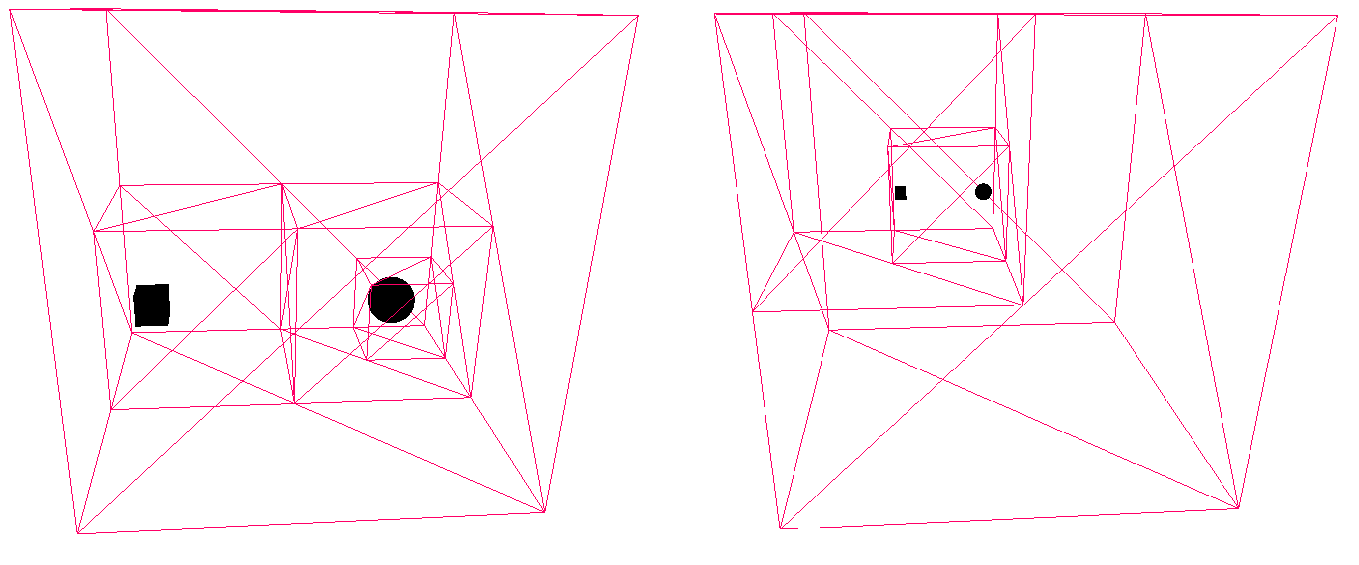
\includegraphics[width=1\linewidth]{images/chapter_navigazione_scena/boxradius.png}\hfill
 \caption[Octree radius.]{A sinistra viene utilizzato radius = 1, a destra radius = 300}
 \label{fig:navigazione_scena_collision_boxradius}
\end{figure}
Nel presente contesto di lavoro ad esso è stato assegnato il valore uguale ad 1, il minimo valore di grandezza possibile. 
Questo per permettere all’oggetto Octree di suddividere lo spazio con il maggior numero di cubi possibili.
\\
Quando infatti il valore radius è elevato, c’è il rischio che il cubo minimo creabile sia grande quanto l’intera scena creata.
\\ 
Di fatto quindi la scena non viene suddivisa e l’algoritmo risulta totalmente inutile, non comportando i miglioramenti di efficienza descritti nel paragrafo \ref{sec:chapter_navigazione_scena_collision_detec}.
\\

Il valore dell’attributo \texttt{undeferred} rappresenta invece un booleano. 
Quando questo valore è false, l’algoritmo rinvia la suddivisione dello spazio fino a quando non viene chiamata la funzione update(). Quando invece è true, la suddivisione dello spazio avviene appena l’oggetto Octree viene istanziato.
\\
Nel presente contesto è stato assegnato ad esso il valore false. Questo permette di avviare la suddivisione chiamando la funzione update solamente quando l’utente avvia la navigazione in prima persona.
\\
Effettuare questo divisione durante la navigazione dall’alto sarebbe inutile, non è detto infatti che l’utente voglia utilizzare la modalità in prima persona.
\\

Il parametro \texttt{depthMax} indica la profondità della scena che l’algoritmo deve considerare per suddividere lo spazio. Un valore troppo basso in scene di elevate dimensioni non permetterebbe di dividere l’intero spazio della scena.
\\
In questo elaborato, a questo attributo è stata assegnata la costante Infinity per permettere la suddivisione di tutto lo spazio. Questo permette di dividere correttamente lo spazio di qualsiasi scena indipendentemente dalla sua dimensione.
\\

Tra tutti, l’attributo fondamentale è \texttt{objectThreshold} che rappresenta il numero di oggetti che devono essere presenti all’interno del cubo affinché la suddivisione avvenga.
Se ad esempio questo parametro viene settato ad 8 e all’interno del cubo nello spazio sono presenti 20 oggetti, allora il cubo viene diviso.
\\
Questa divisione continua fino a quando il cubo contiene un numero di oggetti inferiore alla soglia.
\\

Il parametro \texttt{overlapPct} rappresenta la percentuale di sovrapposizione tra i cubi creati. Il valore minimo è 0 (nessuna sovrapposizione), mentre il massimo è 1 (tutti i cubi sono sovrapposti completamente).

\begin{figure}[htb]
 \centering
 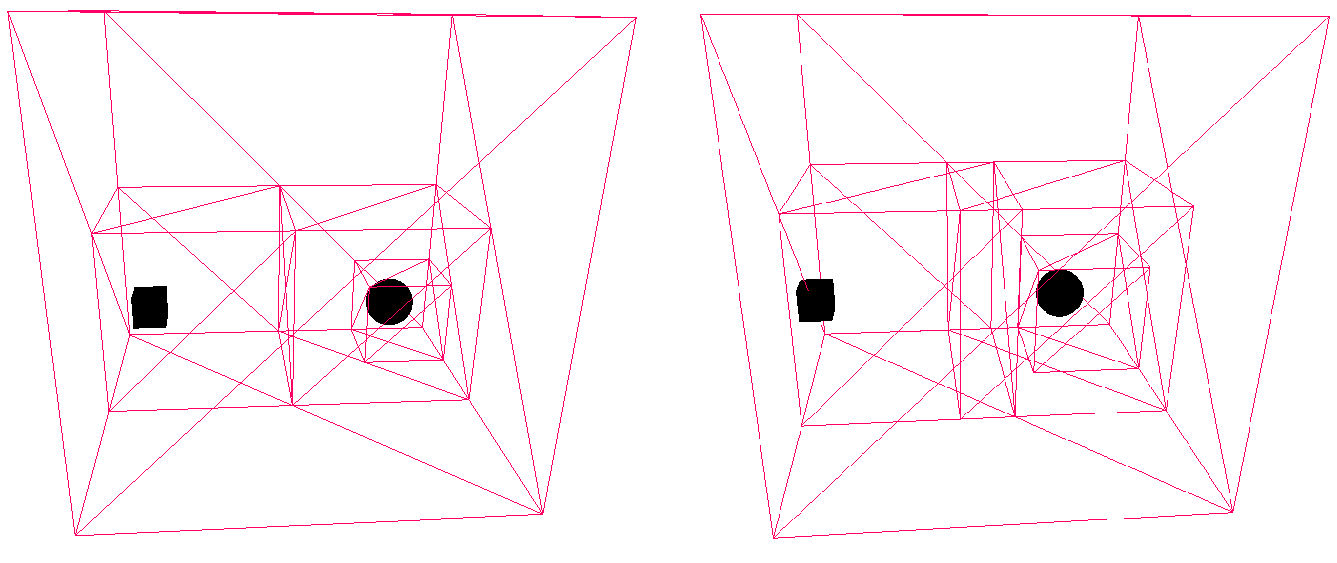
\includegraphics[width=1\linewidth]{images/chapter_navigazione_scena/boxoverlap.png}\hfill
 \caption[Octree overlapPct.]{A sinistra viene utilizzato overlapPct = 0, a destra overlapPct = 0.15}
 \label{fig:navigazione_scena_collision_boxradius}
\end{figure}



Nel presente lavoro è stato assegnato il valore 0.15; una bassa sovrapposizione tra cubi permette infatti di rendere estremamente preciso il calcolo delle intersezioni quando ci sono oggetti che si trovano alle estremità dei cubi di suddivisione. Un valore nullo di sovrapposizione può invece comportare, in alcuni casi, problemi nel corretto riconoscimento delle collisioni.
\\
Quando infatti l’osservatore entra dentro un nuovo cubo di delimitazione, vengono valutate le intersezioni con gli oggetti presenti all’interno di esso (gli oggetti con alta probabilità di collisione).
\\
Può accadere però che questa valutazione avvenga immediatamente dopo che l’osservatore è entrato in contatto con l’oggetto, perchè ubicato proprio alle estremità del cubo. Questo di fatto non permette il riconoscimento della collisione.
\\ 
Il valore di soglia settato a 0.15 risolvere questo inconveniente.
Una volta suddiviso lo spazio vengono quindi lanciati i raggi, descritti in X, a partire dall’osservatore  al fine di calcolare le collisioni all’interno del cubo di divisione.
Ai fini del guadagno di efficienza viene però effettuata una ulteriore accortezza oltre a quelle citate nel paragrafo \ref{sec:chapter_navigazione_scena_collision_detec}: viene istanziato un solo raggio invece dei tredici necessari.
\\ 
Questo unico raggio, per ogni ciclo di render, viene valutato in tutte e 13 le direzioni. 
Una piccola accortezza che soprattutto per architetture di basse prestazione ha permesso di ottenere buoni miglioramenti nella fluidità.
\\
L’osservatore virtuale è in grado di muoversi in una direzione solamente quando l’utilizzatore del sistema preme il pulsante della tastiera che permette quel movimento ed in quella direzione non si trova un ostacolo. Se anche una sola delle due condizioni non viene soddisfatta allora il movimento in quella direzione viene precluso.
\\

Per la mappa, descritta in \ref{sec:caratteristiche_navigatore_mappa} , viene utilizzato un differente renderer a cui è associata una canvas di piccole dimensioni in cui viene disegnata la scena della mappa.
\\
Gli oggetti renderizzati nella mappa vengono associati inseriti in una scena differente da quella utilizzata per gli oggetti mostrati durante la navigazione.
\\
L’utilizzo di due renderer e di due scene differenti ha permesso di disaccopiare la renderizzazione della navigazione da quella della mappa, permettendo agevolmente di avviare e disattivare con estrema facilità la mappa. In particolare quando la mappa viene disattivata, viene anche bloccata la renderizzazione della scena associata alla mappa.
\\
L’ambiente mostrato dalla mappa risulta differente in base al tipo di modalità della mappa scelto e viene utilizzata una camera di tipo Ortographic.
\\
Durante la navigazione in realtà virtuale viene utilizzato l’oggetto \texttt{StereoEffect} che divide la canvas in due parti per permettere la visione stereoscopica 3D \cite{stereo_effect}.
Siccome il navigatore permette l’utilizzo del visore Google Cardboard, viene supposto che questa modalità venga avviata solamente quando il servizio di navigazione viene avviato su smartphone.
\\
In questa modalità non risulta però possibile utilizzare il cellulare tramite i comandi touch in quanto viene inserito all’interno del visore.
\\
Quindi viene sfruttato l’oscilloscopio e l’accelerometro del cellulare tramite la libreria DeviceOrientationControls per modificare il volume di vista in base al movimento della testa dell’utilizzatore del visore.
\\
Il servizio è stato creato in maniera tale da risultare efficiente anche su hardware di basse prestazioni ed il codice è stato strutturato in modo tale da risultare modificabile.